
\documentclass[12pt]{article}
\usepackage[paper=letterpaper,margin=2cm]{geometry}

%\usepackage{coffeestains} %lmao

\usepackage{amsmath}
\usepackage{amsthm} %needed for the proofs 
\usepackage{amssymb}
\usepackage{titling}
\usepackage{thmtools}
\usepackage{mathptmx} %font
\usepackage{verbatim} % for comments
\usepackage{mdframed}
\usepackage[linesnumbered,ruled,vlined]{algorithm2e}
\usepackage{lipsum}

% --- NAMES --- %
\newcommand{\nameone}{Alexandre St-Aubin}
\newcommand{\nametwo}{ and Jonathan Campana}
%images
\usepackage{graphicx}
\graphicspath{ {./images/} }
% to include an image, do: 
%    \begin{center}
%    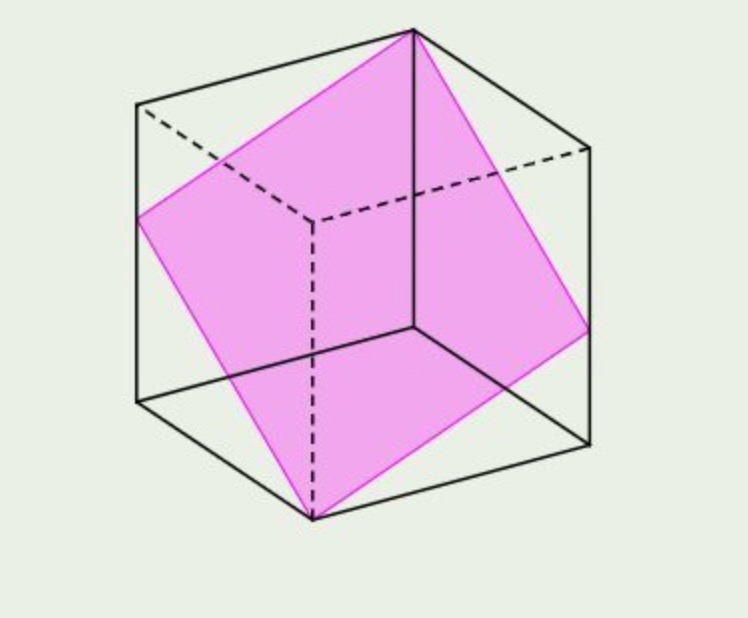
\includegraphics[scale=0.20]{graph.jpg}
%    \end{center}
% OR: 
%\begin{figure}
%    \centering
%    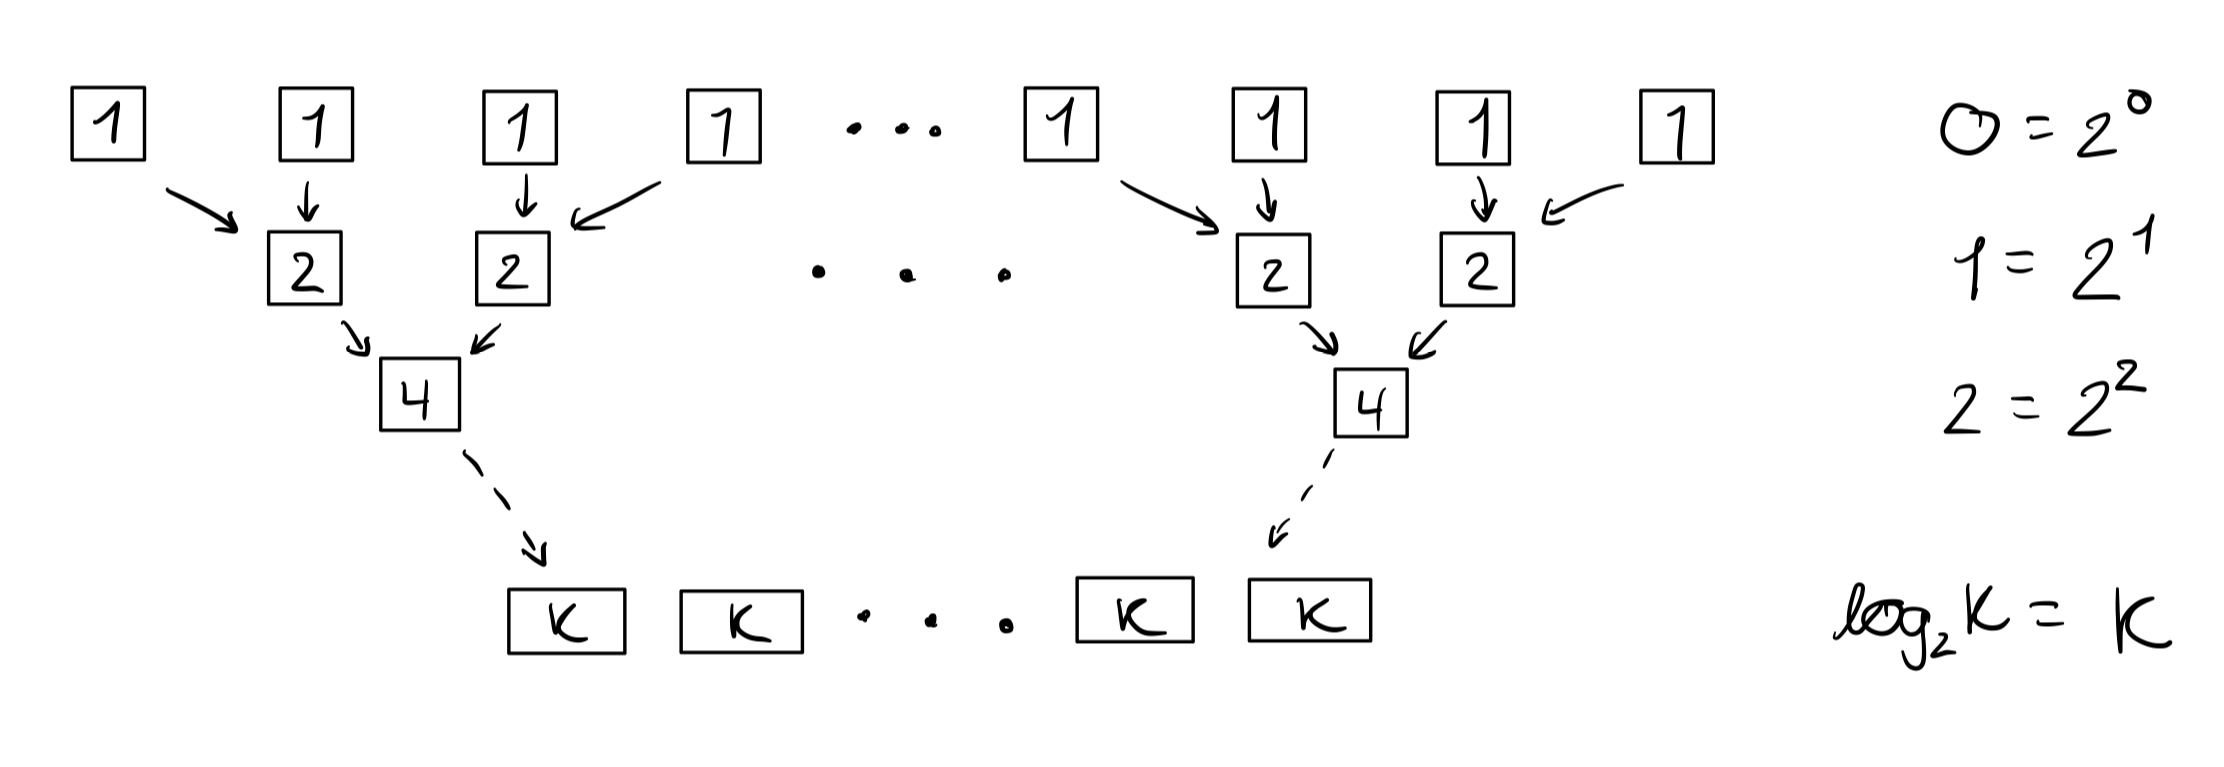
\includegraphics[scale=0.20]{IMG_1052.jpg}
%    \caption{Your caption text here.}
%\end{figure}


%For plots
\usepackage{pgfplots}
\pgfplotsset{compat = newest}

% --- Custom Math Commands --- %
\newtheorem{theorem}{Theorem}
\declaretheoremstyle{lemma}
\declaretheorem[style=lemma, name=Lemma]{lemma}

\theoremstyle{definition}
\newtheorem{definition}{Definition}

\declaretheoremstyle{example}
\declaretheorem[style=example, name=Example]{example}

\theoremstyle{remark}
\newtheorem*{remark}{Remark}

\declaretheoremstyle{proposition}
\declaretheorem[style=proposition, name=Proposition]{proposition}

\declaretheorem[name=Note]{note}
\declaretheoremstyle{note}

\newenvironment{ftheo}
  {\begin{mdframed}\begin{theorem}}
  {\end{theorem}\end{mdframed}}


  % --- Special commands --- %
\newcommand\sol{%
  \\ 
  \\
  \textit{Solution:}\\%
}
% Statistics
\newcommand{\indep}{\perp \!\!\! \perp}
\DeclareMathOperator{\var}{Var}
\DeclareMathOperator{\cov}{Cov}

%Convex optimisation operators
\DeclareMathOperator{\epi}{epi}
\DeclareMathOperator{\lev}{lev}
\DeclareMathOperator{\dom}{dom}
\DeclareMathOperator{\aff}{aff}
\DeclareMathOperator{\ri}{ri}
\DeclareMathOperator{\argmin}{argmin}
\DeclareMathOperator{\conv}{conv}
\DeclareMathOperator{\cl}{cl}


% --- Header --- %
%\renewcommand{\headrulewidth}{.4mm} % header line width

\usepackage[T1]{fontenc} %header
\usepackage[utf8]{inputenc}%header
\usepackage{geometry} %header
\usepackage{fancyhdr}%header
\usepackage{blindtext}
\usepackage{lastpage}

\pagestyle{fancy}
\fancyhf{}
\fancyhfoffset[L]{1cm} % left extra length
\fancyhfoffset[R]{1cm} % right extra length
\rhead{\today}
\lhead{\it \nameone \nametwo}
%\fancyfoot[R]{Page \thepage \hspace{1pt} of \pageref{LastPage}}

% --- Title Page --- % 
\setlength{\droptitle}{-6em}

\title{\textsc{Assignment 4 -- COMP 252}}  
\author{\it \nameone \nametwo}
\date{\today}

\begin{document}
\maketitle 
\thispagestyle{empty} %clear first page numbering
%\coffeestainA{0.9}{0.85}{-25}{5cm}{1.3cm}
\begin{enumerate}
  \item \textsc{Browsing the small elements in a red-black tree}.
  \newpage 
  \item \textsc{Greedy algorithm}. On a flat table, we have placed n disks of radii $r_1, ..., r_n$, numbered from left to right. We push them together without creating overlap, as in the figure below. Give an $O(n)$ time algorithm to compute the size of the smallest axis-aligned rectangle that can hold the disks.
  \sol 

  \begin{algorithm}
    \caption{Greedy circle packing}
    \SetKwProg{Fn}{Function }{\string:}{}
    \SetKwRepeat{Do}{do}{while} %do-while loop macro
    \SetKwInput{KwOut}{Output}
    \SetKwInput{KwIn}{Input}
    \SetKwFunction{rad}{Radius}
    \SetKwFunction{cen}{centre\_dist}
    \SetKwData{dec}{decreasing\_radii}
    \SetKwData{a}{a}
    \SetKwData{b}{b}
    \SetKwData{arr}{array}    
    \SetKwData{ltok}{left\_to\_circle}   
    \SetKwData{maxd}{max\_d}   
    \SetKwData{len}{length}  
    \SetKwData{rm}{remove}   
    \SetKwFunction{makenull}{MAKENULL}
    \SetKwFunction{top}{TOP}
    \SetKwFunction{pop}{POP}
    \SetKwFunction{push}{PUSH}

    \KwIn{An ordered list $\Omega := \{1,2,3,...,n\}$ of $n$ circles. }
    \KwOut{The minimum width of a rectangle that can hold the disks.}
    \BlankLine

    \tcp{\color{blue}returns the radius of the circle a}
    \Fn{\rad{circle \a}}{
        \Return radius of \a;
    }
    \BlankLine

    \tcp{\color{blue}returns the distance between the centres of a and b if they are pushed together.}
    \Fn{\cen{circle \a, circle \b}}{
      \Return $ \sqrt{(\rad(a)+\rad(b))^2 -(\rad(a)-\rad(b))^2};$
    }
    \BlankLine 
    \tcp{\color{blue}largest subarray of $\Omega$ ending with $k$, decreasing in radii. }
    $\dec []\gets new \; \arr \text{ of circles}; $\\
    \BlankLine 
    \tcp{\color{blue}distance from the left side of the rectangle to circle at index}
    $\ltok[] \gets new \; \arr;$\\     
    \BlankLine
    $\ltok[0] \gets 0;$\\ 
    \For{$i\gets 1 \text{ to } n$}{
      \eIf{$i=1$}{
        $\ltok[i] \gets \rad(i);$\\
        $\dec[i] \gets i;$\\ 
      }{
        $\maxd \gets 0;$\\
        \tcp{\color{blue}iterate through array of decreasing radii, starting with the smallest, until larger radius is hit}
        \For{$j \gets \len(\dec)-1 \text{ to } j \gets 0$}{ 
        \tcp{\color{blue}get the distance from the left side of the rectangle to the centre of circle i when it is adjacent to circle at \dec[j]}
          $\maxd \gets \max \{\maxd, \ltok[\dec[j]]+ \cen(\dec[j],i) \}$;\\
          \If{$\rad(i)\geq \rad(j)$}{
            \tcp{\color{blue}if we encounter a circle of larger radius than i, stop checking distances, as there would clearly be an overlap.}
            \text{exit for loop;}
          }
        }
        \tcp{\color{blue} \maxd holds the maximum distance occurring when circle i is adjacent to a circle in \dec. This}
        $\ltok[i] \gets \maxd;$\\ 
        \BlankLine 
        \tcp{\color{blue}update array of decreasing radii.}
        \While{$\rad(i) \geq \rad(\dec[-1])$}{
          $\rm (\dec[-1]);$
        }
        $ \dec[\len(\dec)] \gets i$;\\ 
        }
      }
   \Return \ltok 
    
  \end{algorithm}
\end{enumerate}
\end{document}
